\documentclass[11pt]{article}
\usepackage[margin=0.85in]{geometry}
\usepackage[T1]{fontenc}\usepackage{lmodern,amsmath,amssymb,amsthm,booktabs,graphicx,xcolor,hyperref,eso-pic}
\definecolor{teal}{HTML}{087F8C}\hypersetup{colorlinks=true,urlcolor=teal,linkcolor=teal}
\AddToShipoutPictureBG{\AtPageCenter{\makebox(0,0){\rotatebox{45}{\textcolor[gray]{0.93}{\fontsize{62}{70}\selectfont WORKING PAPER}}}}}
\newtheorem{proposition}{Proposition}
\title{Block Attention for Order-Independent Action Scoring\\\large Independent encoding, a masked architecture, and controlled proofs}
\author{Matthew Dixon, PhD, FRM\\BeliefLens}
\date{20 October 2026 --- Working paper, preliminary experiments}
\begin{document}\maketitle
\begin{abstract}
When an application presents independent action alternatives, their arbitrary list order should not determine their scores. We distinguish two approaches: a tested workaround that independently encodes evidence and actions using a frozen language model, and Block Attention, a single structured-input architecture that restricts attention between blocks, resets positions within blocks, and uses a shared action--evidence scoring head. We give the associated equivariance argument and report tests on Qwen2.5-0.5B, FLAN-T5-base, and a random 22,144-parameter transformer. The experiments establish a structural property on controlled inputs, not accurate financial decisions. Block Attention is a descriptive name for this construction; block masks and permutation-equivariant attention are established concepts, and novelty is not asserted.
\end{abstract}
\section{Two methods, two distinct claims}
\textbf{Independent encoding: tested on pretrained models.} Application code reads one dictionary, encodes evidence separately, and encodes every action description in a separate model call. It reads hidden vectors rather than generating text. A shared, untrained comparison scores each action against the evidence. Separate files are unnecessary. Existing transformer attention remains active within each input.

\textbf{Block Attention: tiny-model proof and a preliminary Qwen readout test.} One structured input contains an evidence block and individually delimited action blocks. Application code identifies these spans, supplies a block attention mask, resets positional indices inside each block, pools each action block and applies a shared scoring head. This is not a prompting instruction and is not implemented merely by writing JSON. It requires control over model internals. A later matched Qwen readout experiment is reported below; useful pretrained-model behavior is not established.

\section{Motivation and prior work}
Option-order sensitivity has been documented in language-model multiple-choice tasks \cite{order}. Deep Sets \cite{deep} and Set Transformer \cite{set} provide established foundations for permutation-invariant and equivariant functions. Our contribution here is an explicit implementation and controlled demonstration of action isolation for a financial workflow. The behavior does not identify a defective attention head or isolate attention from positional encoding and learned behavior as the cause of a pretrained model's failure.
\newpage
\section{The mathematical construction}
Let $X=(E,A_1,\ldots,A_m)$ denote token blocks, where $E$ is evidence and $A_a$ contains an action name and definition. Each token has block ID $b_i$ and within-block position $r_i$. For a causal decoder, define
\begin{equation}
M_{ij}=\begin{cases}0,&b_i=b_j\text{ and }r_j\le r_i,\\-\infty,&\text{otherwise}.\end{cases}
\end{equation}
For each transformer attention head,
\begin{equation}
\operatorname{BA}(X)=\operatorname{softmax}_{\rm row}\left(\frac{QK^\top}{\sqrt{d_k}}+M\right)V.
\end{equation}
The mask forbids cross-block attention. It does \emph{not} suffice alone: token representations must use local positions $r_i$, not their global positions in the concatenated prompt. With learned positional embeddings, initialize $h_i^{(0)}=e(t_i)+p(r_i)$. With rotary or other position mechanisms, their indices and any relative biases must respect block-local coordinates too. The mask must hold in every layer; residuals, feed-forward networks and normalization must not mix blocks.

Let $F_\theta$ be the frozen transformer. Normalize evidence-token rows to obtain $H\in\mathbb R^{n_E\times d}$. Independently pool and normalize each action block:
\begin{equation}
q_a=\operatorname{norm}\left(\frac{1}{|A_a|}\sum_{i\in A_a}h_i^{(L)}\right).
\end{equation}
The exact untrained head used in our tests is
\begin{equation}
w_a=\operatorname{softmax}(Hq_a),\quad z_a=H^\top w_a,\quad
s_a=q_a^\top z_a,\quad c_a=\frac{\exp s_a}{\sum_b\exp s_b}.
\end{equation}
There are no additional learned projections or fitted temperatures. $c_a$ is a normalized compatibility score, not a language-generation probability or calibrated belief. Evidence and action blocks first remain isolated; the explicit head subsequently allows action--evidence interaction.

\begin{proposition}
Assume fixed tokenization within blocks, shared weights, local positions, the mask above at every layer, tokenwise residual/normalization/feed-forward operations, and deterministic inference. Permuting action blocks permutes their score rows: $S(E,PA)=PS(E,A)$. Named-action scores are invariant in exact arithmetic.
\end{proposition}
\begin{proof}
Local positions make each block's initial representations independent of its concatenation position. The mask restricts every attention sum to the same within-block tokens. By induction over layers, each block has the same hidden states under reordering. Shared pooling and action--evidence comparison therefore preserve the same named-action score. The denominator is symmetric in the action scores.
\end{proof}
In software, normalize in canonical action-name order and use an order-independent tie-break. Use tolerances for floating-point changes. Ordinary autoregressive answer generation is not covered by the proposition; an output token attending across blocks can reintroduce order sensitivity. Evidence-record order and action paraphrases are also outside the guarantee.
\newpage
\section{Pretrained-model workaround: measured results}
\subsection*{Preliminary results: frozen pretrained models}
Five constructed EPS cases cover above/below/equal consensus, missing actual EPS and conflicting actual EPS. Actions are BUY, CASH and WITHHOLD, not BUY/HOLD/SELL. Each case has six action orders and five identical repeats: 150 evaluations per method. There are 75 within-case pairs of distinct orders and 300 within-case/order pairs of repeats. These are five independent input scenarios, not 150 independent financial observations.

The prompt baseline serializes the dictionary into one input. All three candidate answers are teacher-forced and their token log probabilities summed, including EOS. Scores are normalized over those three complete answers. Qwen was also scored without EOS as a control. No independent generated-answer evaluation was performed in this experiment. The alternative uses independently encoded representations and Equation (4).
\begin{center}\small
\begin{tabular}{llrr}\toprule
Model & Measure & JSON prompt & Separate encoding\\\midrule
Qwen 0.5B & Mean order TV & 0.2505 & 0\\
 & Maximum order TV & 0.5975 & 0\\
 & Changed top rank / 75 & 32 & 0\\
 & Maximum repeat TV & 0 & 0\\\midrule
FLAN-T5-base & Mean order TV & 0.0546 & 0\\
 & Maximum order TV & 0.1488 & 0\\
 & Changed top rank / 75 & 0 & 0\\
 & Maximum repeat TV & 0 & 0\\\bottomrule
\end{tabular}\end{center}
Here $\operatorname{TV}(p,q)=\tfrac12\sum_a|p_a-q_a|$. Qwen used 494,032,768 parameters and 111.93 seconds on CPU; FLAN used 247,577,856 parameters and 51.64 seconds. Weights were frozen. CPU float32 inference was deterministic. Repeated inputs were recomputed; invariant results were not returned from an answer cache. In Qwen, removing EOS still gave 32 changed rankings and maximum TV 0.5969.

\section{Direct Block Attention proof: tiny-model ablations}
\subsection*{Preliminary results: masked tiny transformer}
A two-layer transformer with width 32, four attention heads, tokenwise layer normalization and a 64-unit feed-forward hidden layer has 22,144 parameters. All weights are random and fixed (seed 20261020). The same five-case/six-order/five-repeat design compares three conditions with identical weights and the same pooling/scoring head.
\begin{center}\small
\begin{tabular}{lrrr}\toprule
Condition & Max. order TV & Changed ranks / 75 & Max. forbidden attention\\\midrule
Ordinary causal attention & 0.04117 & 52 & 0.96843\\
Block mask, global positions & 0.04879 & 51 & 0\\
Block mask, local positions & 0 & 0 & 0\\\bottomrule
\end{tabular}\end{center}
All repeat distances were zero. In the full Block Attention condition, changing an earlier BUY description, including its length, changed the CASH vector by exactly zero. All forbidden attention entries in both layers were zero. Tests asserted invariance within $10^{-6}$; measured differences were zero. The mask-only ablation demonstrates why global positions must also be removed. This is an architectural test on one random initialization, not a trained small language model or pretrained-model retrofit.
\newpage
\section{Interpretation, implementation and limits}
The practical workaround bypasses the vocabulary output head and decoding, not attention within the model. Block Attention changes the attention connectivity of a single structured input. Both methods isolate action representations before a shared evidence comparison. The tiny-model proof does not establish that a mask retrofit preserves useful pretrained representations.

The stipulated EPS policy was matched on 60/150 Qwen runs in each method and 30/150 FLAN runs in each method. We did not optimize decision accuracy, train a scoring head, test returns, or use independent investment-outcome labels. The purpose is solely to establish action-order behavior. The baseline probabilities and alternative compatibility scores have different meanings; their absolute levels are not interchangeable. Independent repeats rule out observed run-to-run variation on this setup, not population-wide instability or hardware effects.

A production implementation must specify trusted parsing of action boundaries, position handling, padding and cache isolation, the scope of normalization, a shared head, an order-independent tie policy, and numerical tolerances. Learned cross-action attention could be included if it is permutation equivariant; isolation is a sufficient construction, not the only solution. Dependent action plans should not be treated as an unordered choice set.

\section{Reproduction artifacts}
\begin{itemize}
\item \texttt{dictionary\_invariance/run.py}: FLAN independent-encoding comparison.
\item \texttt{dictionary\_invariance/qwen/run.py}: Qwen comparison with EOS and prefix scores.
\item \texttt{block\_attention/run.py}: tiny model, masks, positional ablation and isolation test.
\item Each directory includes machine-readable outputs and \texttt{summary.json}.
\end{itemize}
Model revisions:\par
Qwen: \texttt{7ae557604adf67be50417f59c2c2f167def9a775}.\par
FLAN: \texttt{7bcac572ce56db69c1ea7c8af255c5d7c9672fc2}.\par The recorded environment uses PyTorch 2.13.0 and Transformers 4.57.3 for pretrained models. Tiny-model execution takes approximately 0.15 seconds after imports on this CPU; it is not a training-time estimate.

\begin{thebibliography}{9}
\bibitem{order} P. Pezeshkpour and E. Hruschka (2024). Large Language Models Sensitivity to the Order of Options in Multiple-Choice Questions. Findings of NAACL. \url{https://aclanthology.org/2024.findings-naacl.130/}
\bibitem{deep} M. Zaheer et al. (2017). Deep Sets. NeurIPS. \url{https://arxiv.org/abs/1703.06114}
\bibitem{set} J. Lee et al. (2019). Set Transformer: A Framework for Attention-based Permutation-Invariant Neural Networks. ICML. \url{https://proceedings.mlr.press/v97/lee19d.html}
\end{thebibliography}
\newpage
\section{Explicit set semantics and repeated-number tests}
An application must distinguish an unordered sample from an ordered sequence explicitly. For example:
\begin{verbatim}
{"type": "set", "items": [0.12, -0.83, 1.47],
 "duplicates": "preserve"}
\end{verbatim}
Here ``set'' denotes a multiset of observations: repeated values are retained. A schema compiler assigns each item a separate block and local positional coordinates, followed by symmetric pooling. A sequence declaration instead preserves sequence positions and the ordinary attention pathway. The caller supplies the semantics; the model does not infer exchangeability, independence or chronology from values. Within-record order may still matter for structured or textual items. The implementation rejects missing semantics and non-finite inputs.

\subsection*{Preliminary results: fixed 50-number samples}
We generated twenty fixed samples of fifty independent standard-normal pseudorandom draws. For each sample, every comparison reuses exactly those fifty values: the identity ordering plus ninety-nine permutations, each repeated ten times. An assertion checks that the sorted input values agree exactly after every permutation. Across three configurations this gives 60,000 evaluations. Additional samples are replication checks, not replacements for the fixed-input comparisons.

An untrained two-layer, four-head, width-32 transformer (18,785 parameters) embeds each scalar with a linear map, adds positions, applies its layers, averages the hidden vectors and applies a fixed random linear readout:
\[
y_\pi=w^\top\left(\frac1{50}\sum_{i=1}^{50}h_i(x_\pi)\right)+b.
\]
This output is a diagnostic, not an estimated population statistic. Across the first fixed sample, ordinary causal attention yields an output range of 0.14754; block masking with global positions yields 0.04558; block masking with local positions yields exactly zero. Across all twenty samples the corresponding maximum ranges are 0.18770, 0.06765 and zero. Every repeated-input range is zero. Permuting items only permutes the final hidden vectors under the full construction: measured equivariance error is zero.

Each number is represented by one continuous embedding, so a singleton block's attention is trivial (self-only). This is a deliberate architectural isolation test and reduces to shared per-item processing plus symmetric pooling. It does not establish gains from learned attention. Changing the first sample's values by adding one changes the full construction's output by 0.20905; this separate control confirms that the output is not constant in its values. The ordering comparisons never change values.
\newpage
\section{An interpretable outcome: arithmetic mean}
To make the diagnostic intuitive, consider an explicitly constructed one-head calculation with $Q=K=0$, $V_i=x_i$, no positional embeddings, residuals or feed-forward network, and arithmetic-mean pooling. Softmax assigns uniform weights to each row's allowed inputs. The target is the ordinary sample mean $\bar x=\frac1n\sum_i x_i$.

With ordinary causal masking, each row averages its visible prefix. Pooling those averages gives
\[
y_{\rm causal}(x_\pi)=\frac1n\sum_{i=1}^n\frac1i\sum_{j=1}^i x_{\pi(j)}
=\sum_{j=1}^n\left(\frac1n\sum_{i=j}^n\frac1i\right)x_{\pi(j)}.
\]
Earlier items receive larger effective weights. This is generally not the sample mean, and changing which number occupies each position changes the result. For singleton Block Attention, each row sees only itself, so $h_i=x_{\pi(i)}$ and
\[
y_{\rm block}(x_\pi)=\frac1n\sum_i x_{\pi(i)}=\bar x.
\]
An important control removes the causal restriction altogether. Every row then averages all numbers uniformly; pooling also returns $\bar x$. Thus Block Attention is sufficient here, not necessary. Reading the final causal prefix alone would also recover the mean. The example isolates aggregation and visibility choices, not an inherent inability of attention to calculate means.

\subsection*{Preliminary results: same numbers, different order}
The first sample has true mean $-0.0736113354$. The exact same fifty numbers give:
\begin{center}
\begin{tabular}{lrr}\toprule
Calculation & Original order & Shuffled order\\\midrule
Causal prefix attention + pooling & 0.081649 & -0.056449\\
Singleton Block Attention + pooling & -0.073611 & -0.073611\\
Unrestricted uniform attention + pooling & -0.073611 & -0.073611\\\bottomrule
\end{tabular}
\end{center}
Across one hundred permutations of this sample, the causal output spans $[-0.34655,0.28677]$. Both invariant constructions return the exact mean in every tested order. Twenty fixed samples, one hundred orders, ten repetitions and three configurations give 60,000 evaluations. Every repeat is identical; no training or randomness in execution is involved. The maximum causal absolute error across all samples and orders is 0.47787; the other two constructions have zero measured error. These are analytic demonstrations, not a fitted estimator or evidence of trained-model competence.

\newpage
\section{A natural-language counting control: stable but incorrect}
We tested whether an ordinary pretrained model changes a familiar statistical answer when unordered numerical observations are shuffled. One fixed sample of fifty synthetic clinic waiting times was drawn once using seed 20261022. Nineteen values exceed thirty minutes, so the correct response is ``NO; count=19; percentage=38\%.'' The same values were reused in ten permutations and three identical repeats, with the question and answer-label order held fixed. The execution order was randomized and the manifest frozen before inference. No calculator or expected answer was supplied to Qwen2.5-0.5B-Instruct.

All thirty unconstrained greedy responses were identical: ``NO; count=50; percentage=0\%.'' They were validly formatted and untruncated. The NO answer was correct, but the count and percentage were wrong and internally inconsistent. This is a counting/instruction failure, not observed order-induced answer instability. Exact response accuracy was zero of thirty.

Teacher-forced YES/NO prefix scores excluding EOS gave conditional YES probabilities between 0.23746 and 0.26800, a range of 3.0534 percentage points. These scores condition on the two candidate prefixes and are not truth probabilities. Identical-prompt repeats yielded zero numerical or text variation. The run took 49 seconds on CPU with float32 eager inference, neutral repetition penalty and greedy decoding. No sampling or training occurred.

This negative finding for final-answer sensitivity is retained alongside the positive order-effect experiments. It does not show broad robustness: only one fixed numerical sample and one small model were tested. Nor does it show Block Attention repairing a meaningful counting task: that comparison has not been trained or performed. Reproduction files are in \texttt{waiting\_times/}, including the manifest and raw outputs.

\newpage
\section{Matched pretrained Qwen readout with Block Attention}
A follow-up applies a restricted attention graph directly to frozen Qwen2.5-0.5B, retaining its vocabulary output head. The same fifty waiting times, ten orders and three repeats are used in each of three configurations. Numbers are serialized as identically formatted records, with fixed segment tokenization. This differs from the earlier JSON list, so a new matched ordinary baseline is required. Input-token hashes are identical across configurations within each ordering. Ninety calls took 58.21 seconds on CPU.

The instruction prefix uses ordinary causal attention. Each numerical record can see that prefix and its own earlier tokens, but no other numerical record. The fixed assistant/readout suffix can see the prefix, all records and its own earlier suffix tokens. The full construction resets each record's rotary positions to prefix length plus within-record index; prefix and suffix positions stay fixed. This directed extension of Block Attention lets the answer read the full set without letting records acquire contexts dependent on their list position. Its suffix representations are permutation invariant in exact arithmetic by the same layerwise symmetry argument, subject to the stated mask and positional conditions.

The original output head scores the single-token uppercase candidates YES and NO at the final assistant-prefix token. These are normalized candidate probabilities, not compatibility scores. No answer is generated for this comparison.
\begin{center}\small
\begin{tabular}{lrrr}\toprule
Configuration & Min. $P(\mathrm{YES})$ & Max. $P(\mathrm{YES})$ & Range (percentage points)\\\midrule
Ordinary causal & 21.734693\% & 23.566553\% & 1.831860\\
Restricted mask, global positions & 9.217633\% & 9.741331\% & 0.523698\\
Restricted mask, local positions & 19.726548\% & 19.726937\% & 0.000389\\\bottomrule
\end{tabular}\end{center}
Every identical-repeat difference was zero. The full construction's range is $3.89\times10^{-6}$ in probability units, within the declared $10^{-5}$ numerical tolerance. It is not bitwise invariant. Masked attention entries were zero in audited order-zero runs across every layer, and the readout's access to all records was checked. The residual is consistent with floating-point reduction effects; a higher-precision diagnosis was not conducted.

\textbf{Critical qualification.} Uppercase YES and NO together receive 95.71--96.77\% of raw probability mass in the ordinary condition, but only 8.6926--8.6929\% under the full mask/local-position construction. Although NO remains first within the two uppercase candidates, the unconstrained vocabulary argmax becomes title-case \texttt{Yes} in all thirty full-construction runs. In the mask-only condition it is NO in twenty-four runs and COUNT in six. Thus invariant conditional scores do not establish preserved output behavior, calibration or counting accuracy. A mask retrofit can substantially alter the pretrained model's distribution. This experiment is an architectural readout check on one fixed sample, not a validated counting solution. Raw results and code are in \texttt{waiting\_times/block\_matched/}.

\newpage
\section*{Figure 1: the tested independent-encoding workaround}
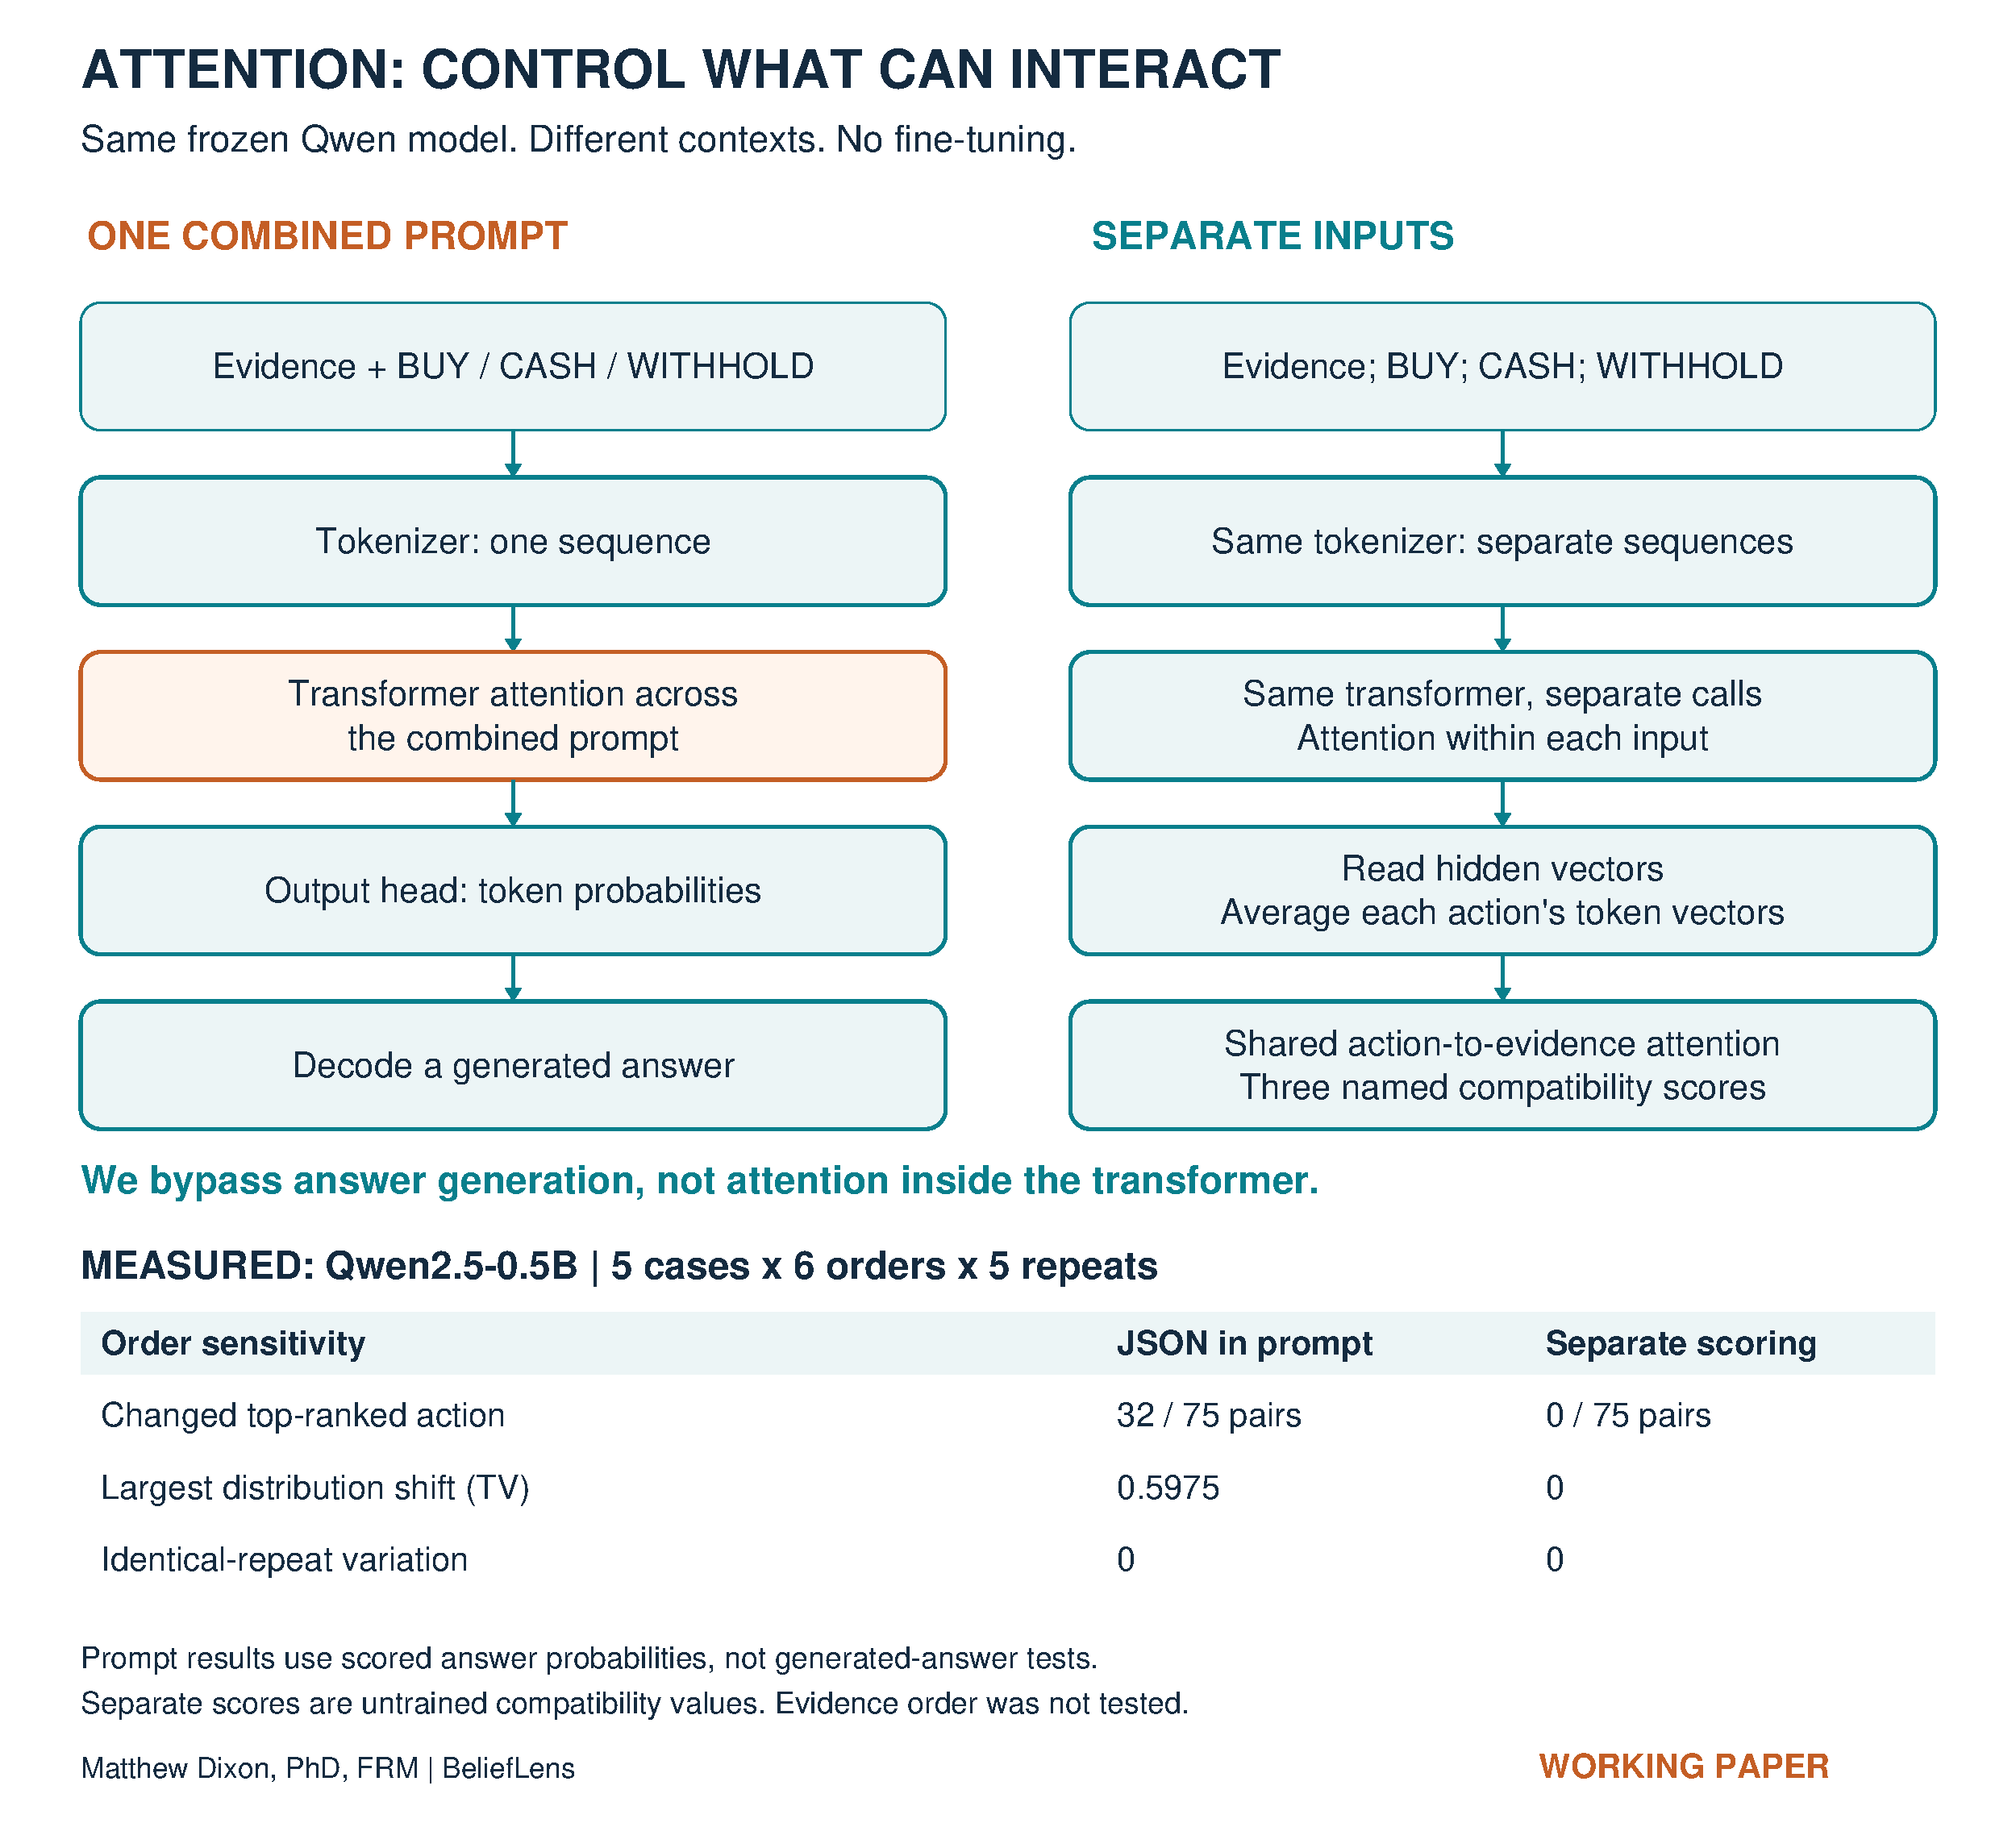
\includegraphics[width=\linewidth]{partial_attention_figure.pdf}
\newpage
\section*{Figure 2: Block Attention and its positional ablation}
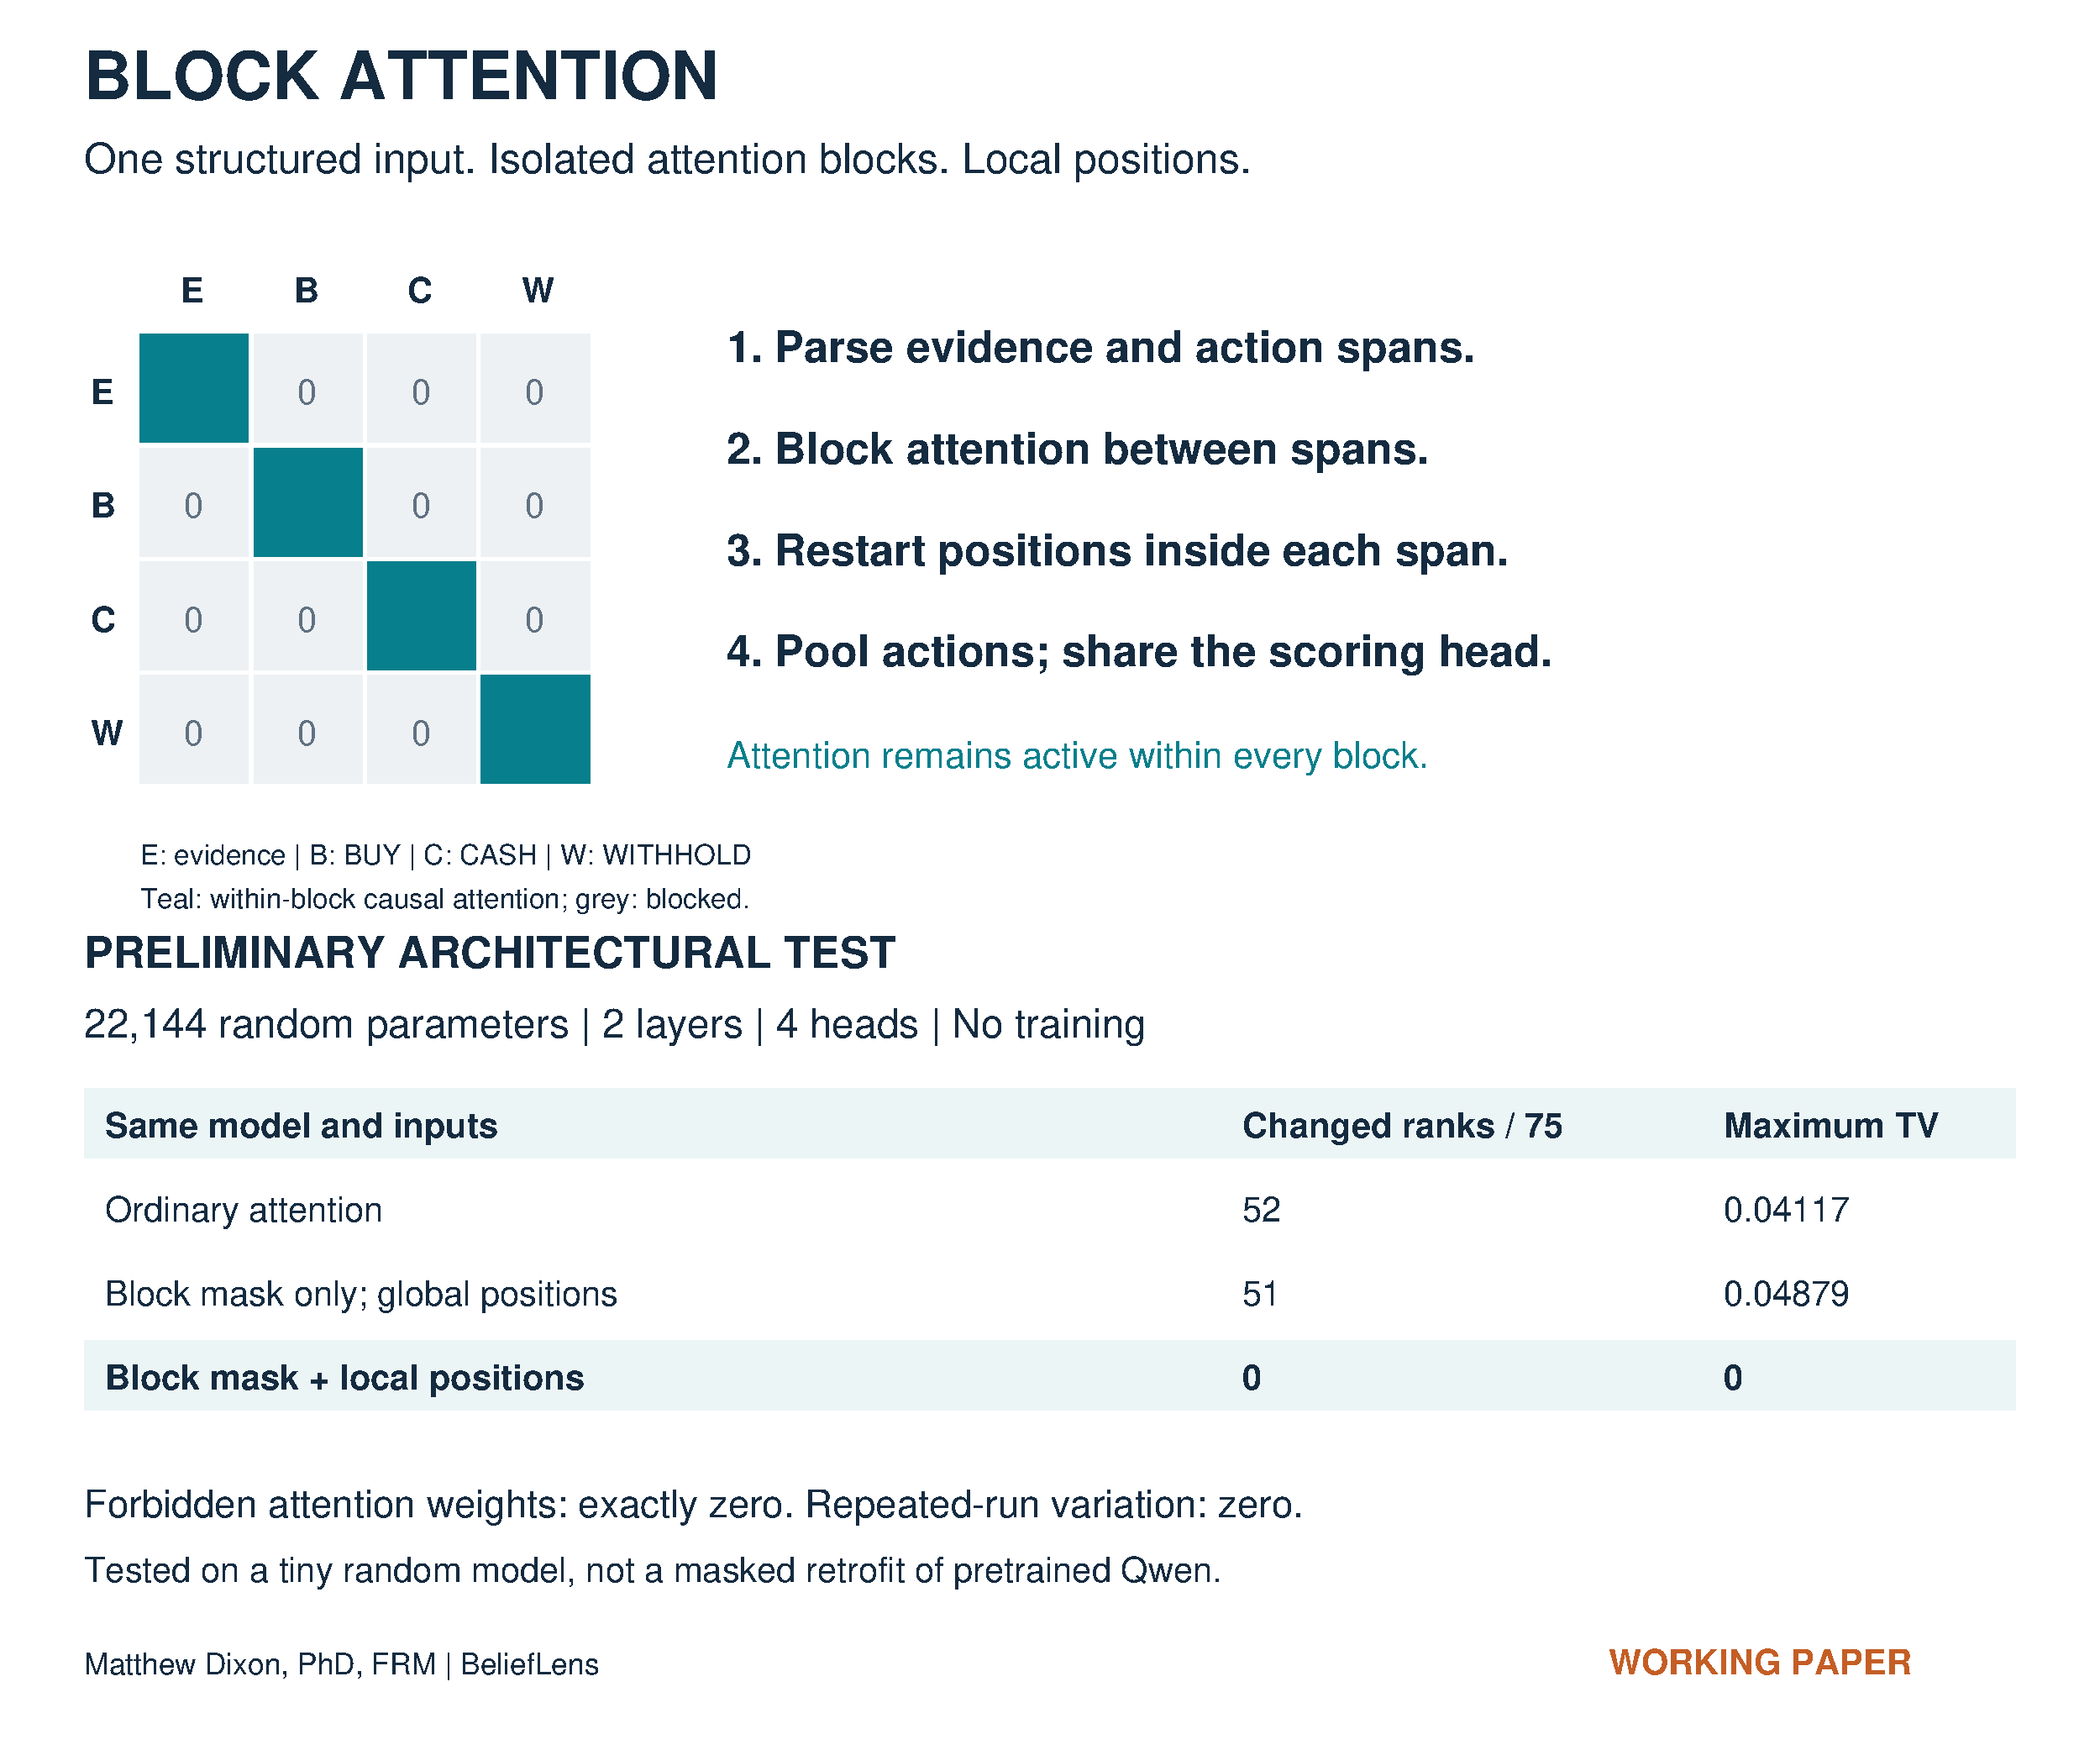
\includegraphics[width=\linewidth]{block_attention_figure.pdf}
\end{document}
